\begin{figure}[htb]
\begin{center}
(a)\hspace{1cm}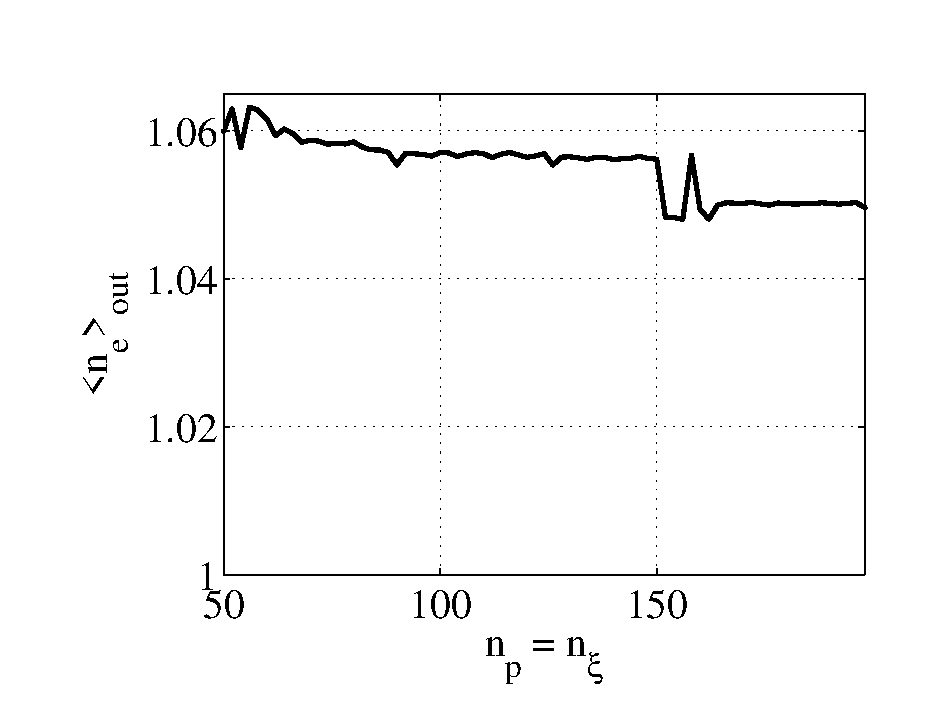
\includegraphics[width = 2in,height = 1in]{figures/test4_np_nmhu_010_neout.eps}\\
(b)\hspace{1cm}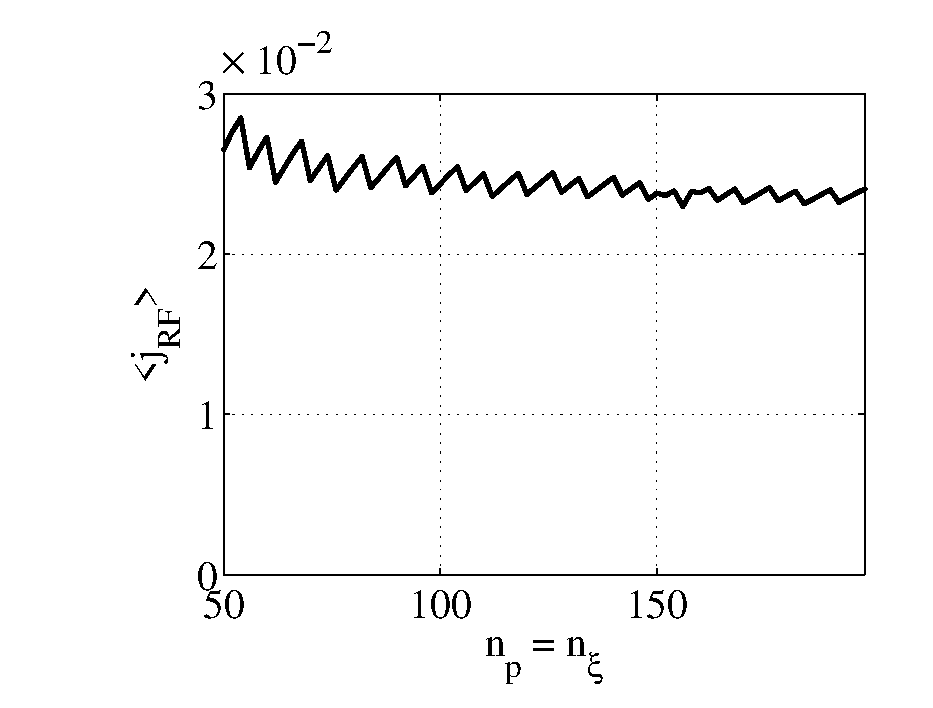
\includegraphics[width = 2in,height = 1in]{figures/test4_np_nmhu_010_j.eps}\\
(c)\hspace{1cm}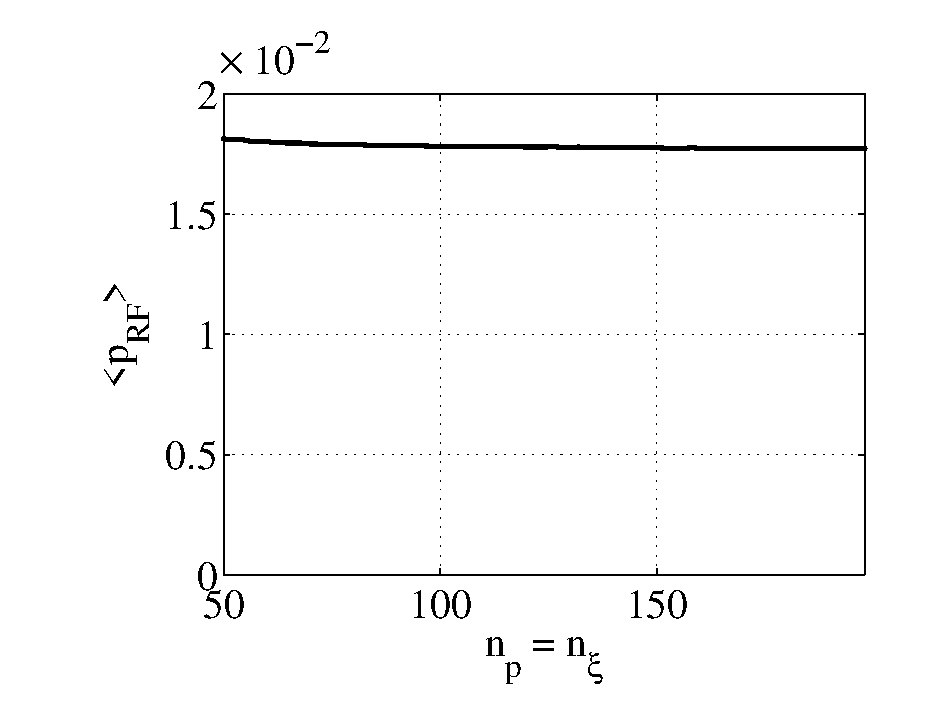
\includegraphics[width = 2in,height = 1in]{figures/test4_np_nmhu_010_p.eps}\\
(d)\hspace{1cm}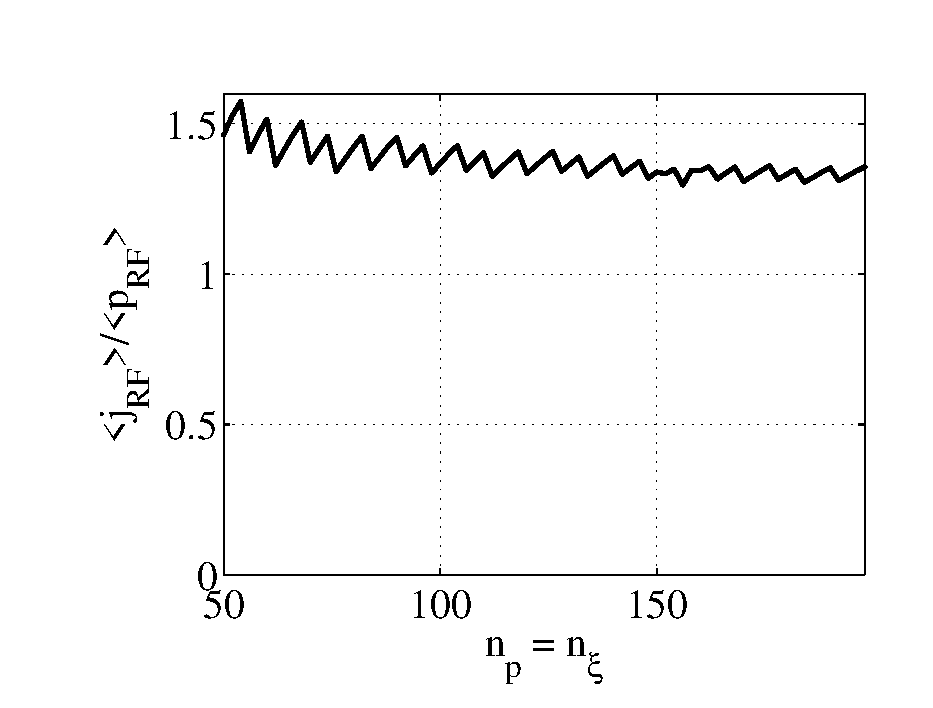
\includegraphics[width = 2in,height = 1in]{figures/test4_np_nmhu_010_eta.eps}\\
(e)\hspace{1cm}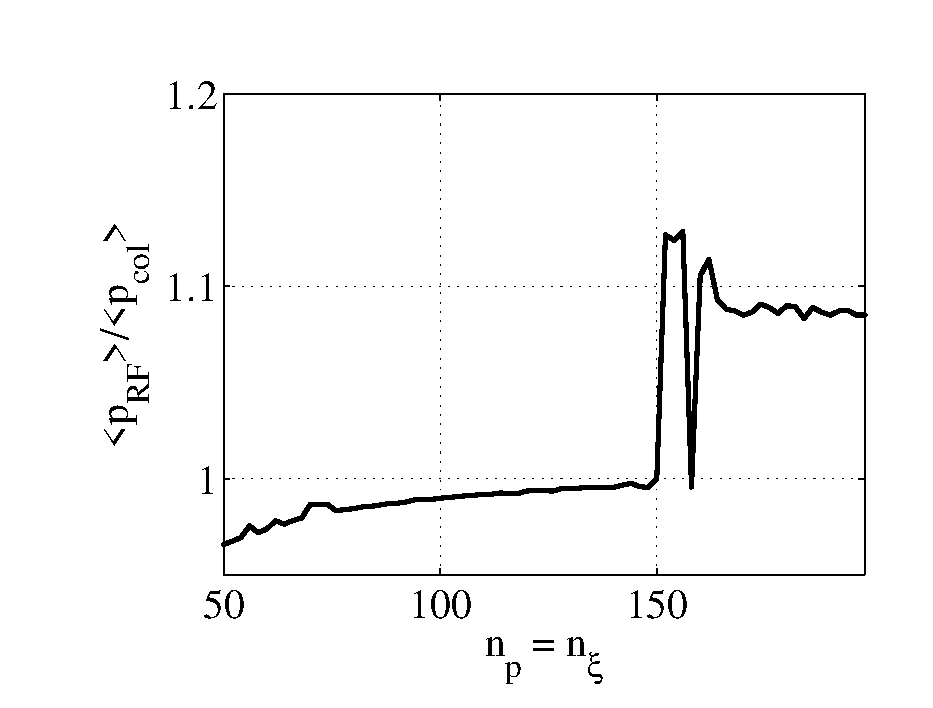
\includegraphics[width = 2in,height = 1in]{figures/test4_np_nmhu_010_rf_col.eps}\\
\caption{ECCD in DIII-D ($\rho = 0.1,\ D_{\text{EC}} = 0.15,\
N_{\parallel} = 0.3,\ Y = 0.98$). Output density (a), normalized
current density (b), normalized absorbed power density (c),
normalized current drive efficiency (d), ratio of power absorbed
to power lost on collisions (e), as a function of grid size ($n_p
= n_{\xi}$).}
%\label{ebw_es}
\end{center}
\end{figure}

\begin{figure}[htb]
\begin{center}
(a)\hspace{1cm}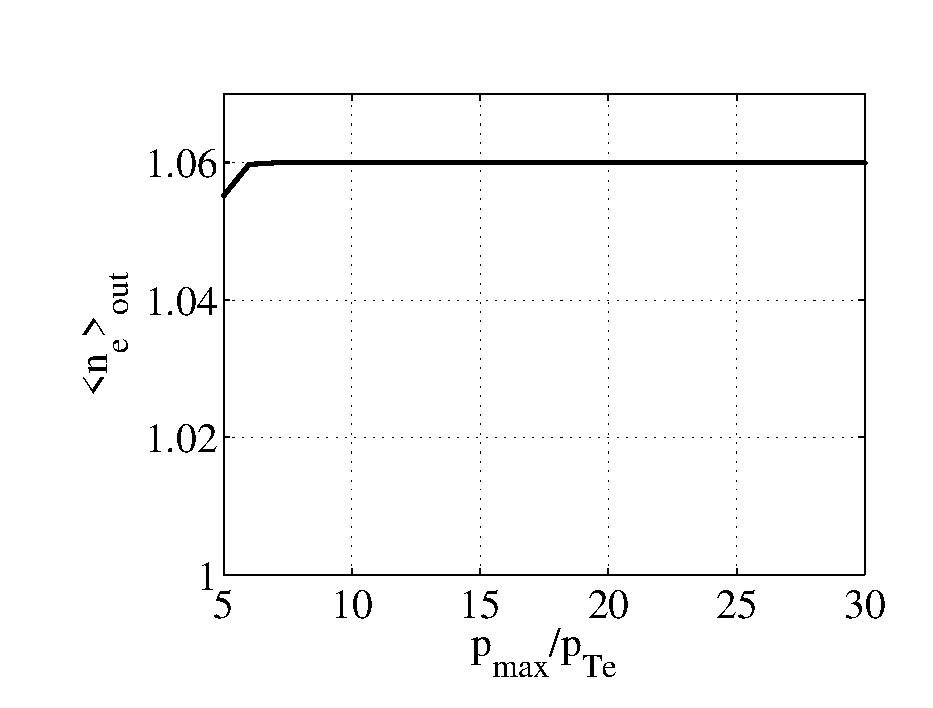
\includegraphics[width = 2in,height = 1in]{figures/test4_pmax_010_neout.eps}\\
(b)\hspace{1cm}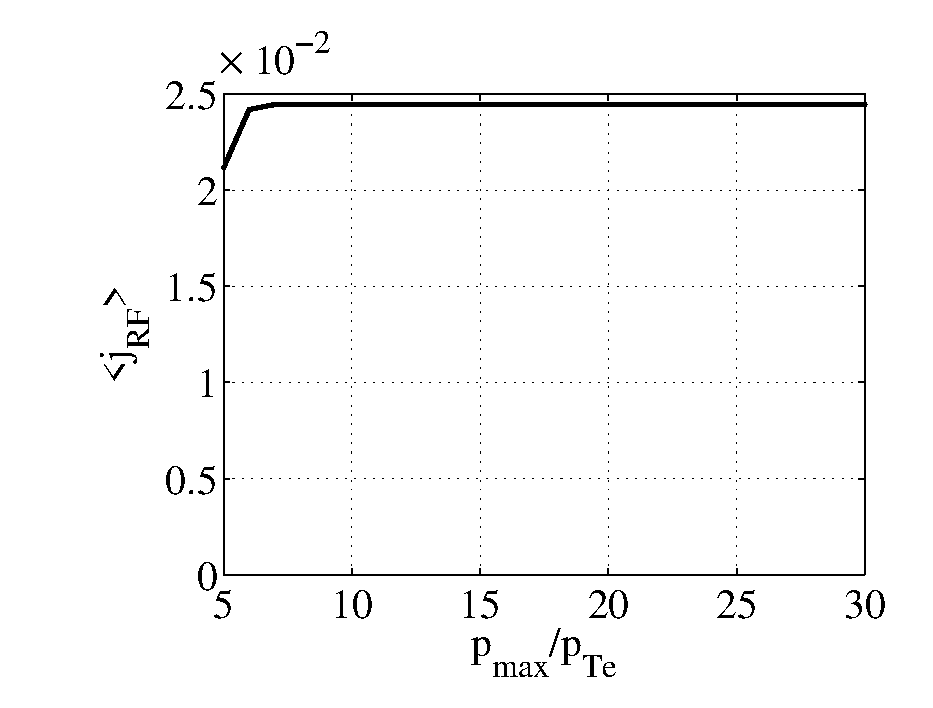
\includegraphics[width = 2in,height = 1in]{figures/test4_pmax_010_j.eps}\\
(c)\hspace{1cm}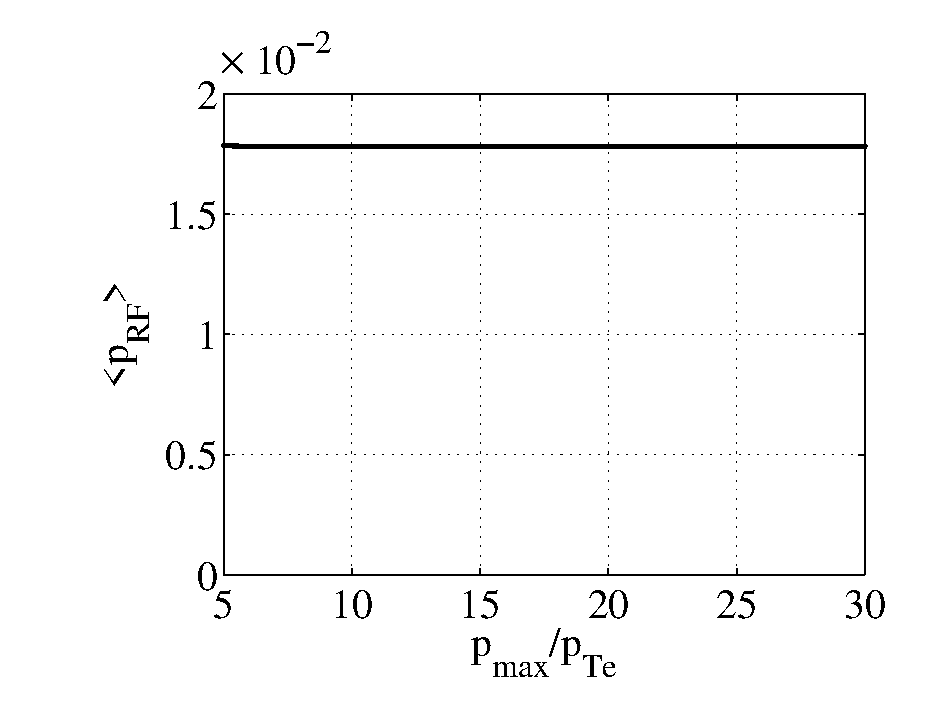
\includegraphics[width = 2in,height = 1in]{figures/test4_pmax_010_p.eps}\\
(d)\hspace{1cm}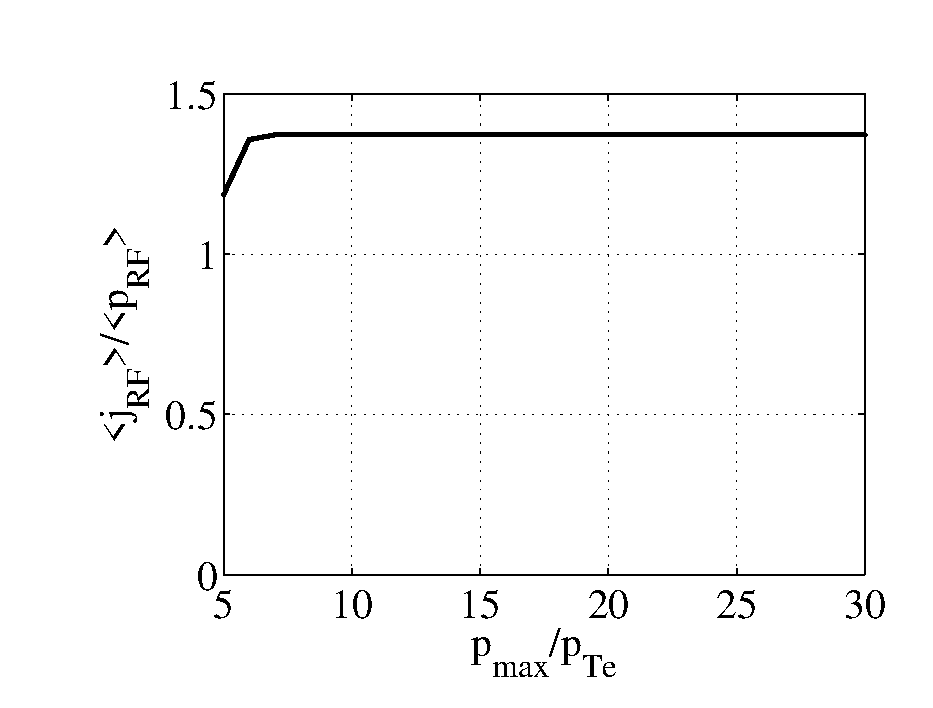
\includegraphics[width = 2in,height = 1in]{figures/test4_pmax_010_eta.eps}\\
(e)\hspace{1cm}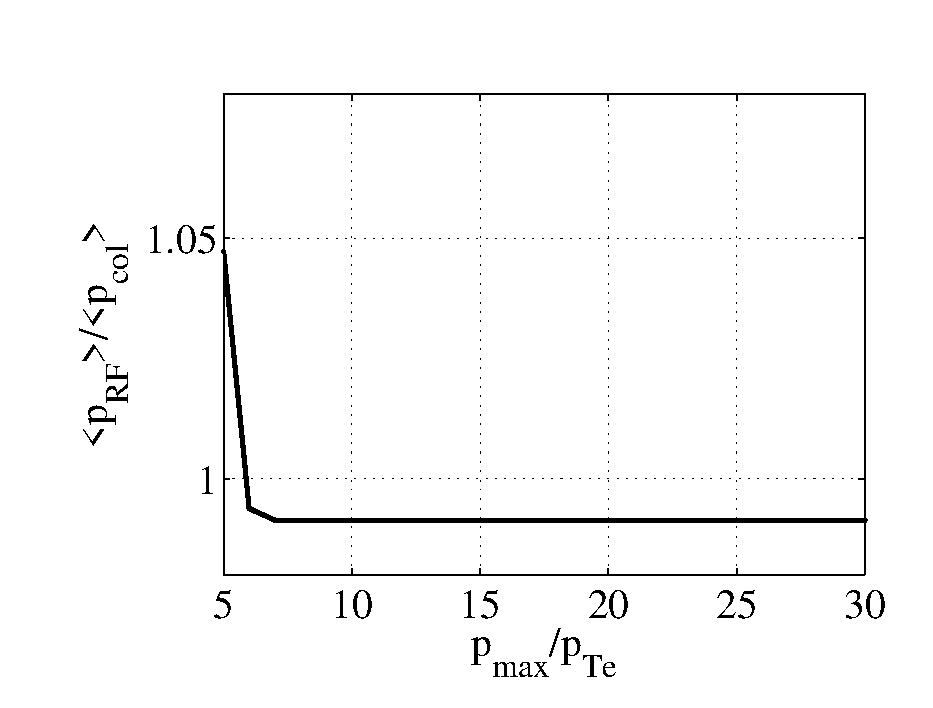
\includegraphics[width = 2in,height = 1in]{figures/test4_pmax_010_rf_col.eps}\\
\caption{ECCD in DIII-D ($\rho = 0.1,\ D_{\text{EC}} = 0.15,\
N_{\parallel} = 0.3,\ Y = 0.98$). Output density (a), normalized
current density (b), normalized absorbed power density (c),
normalized current drive efficiency (d), ratio of power absorbed
to power lost on collisions (e), as a function of momentum grid
limit $p_{\max}$ ($n_p = 10p_{\max},\ n_{\xi} = 100$).}
%\label{ebw_es}
\end{center}
\end{figure}

\begin{figure}[htb]
\begin{center}
(a)\hspace{1cm}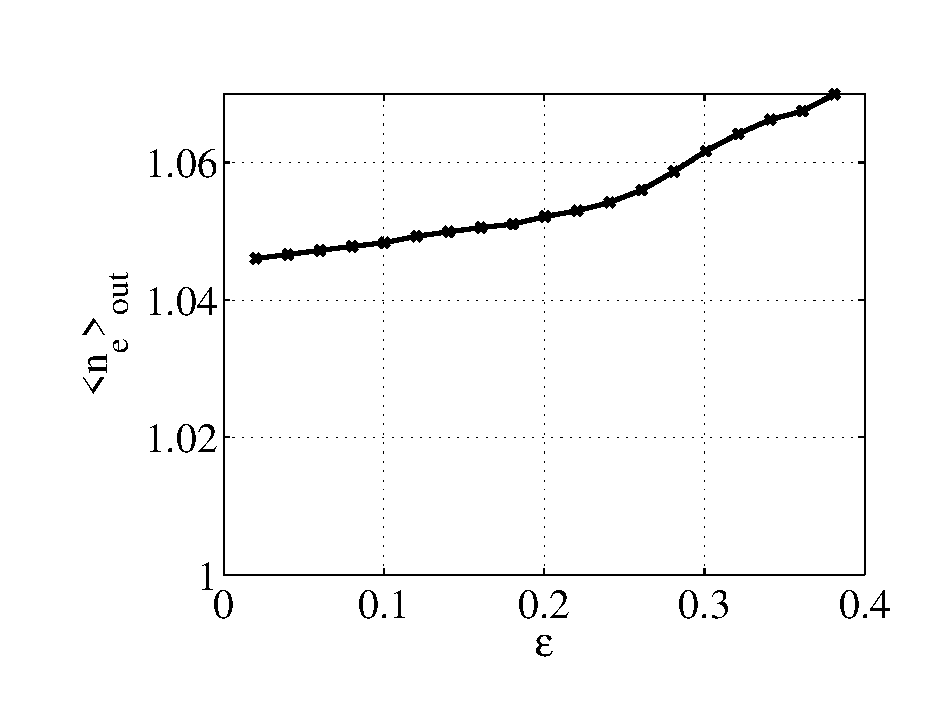
\includegraphics[width = 2in,height = 1in]{figures/test4_CST_ia_neout.eps}\\
(b)\hspace{1cm}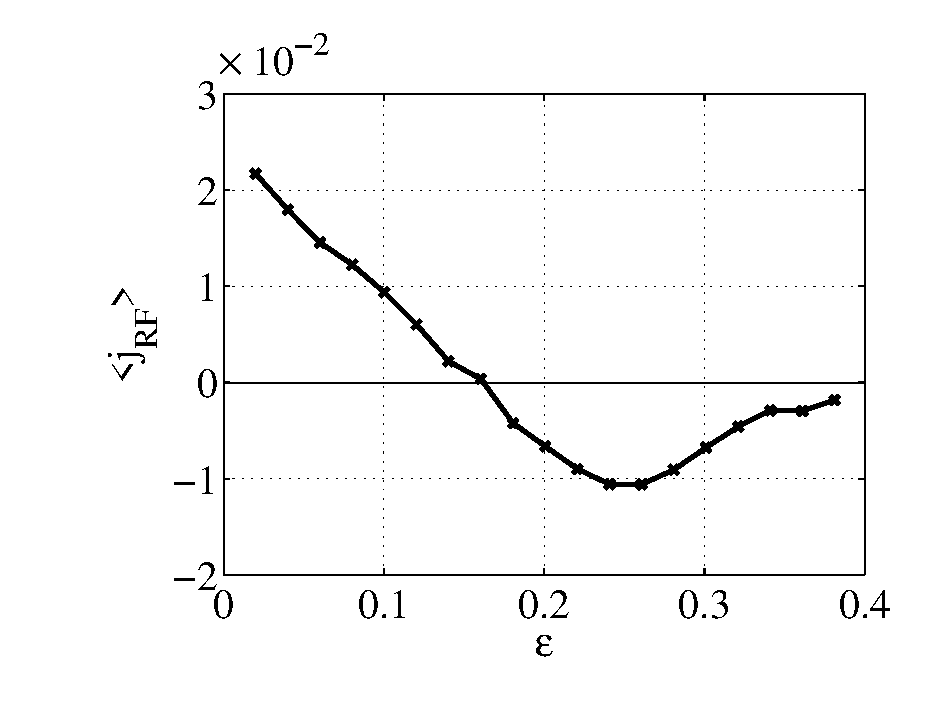
\includegraphics[width = 2in,height = 1in]{figures/test4_CST_ia_j.eps}\\
(c)\hspace{1cm}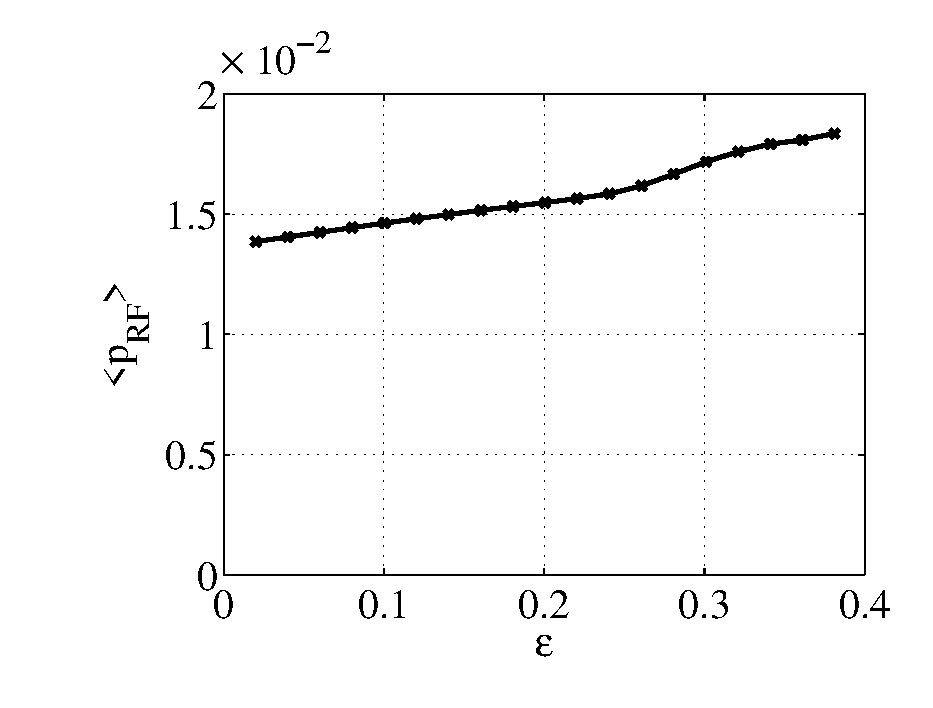
\includegraphics[width = 2in,height = 1in]{figures/test4_CST_ia_p.eps}\\
(d)\hspace{1cm}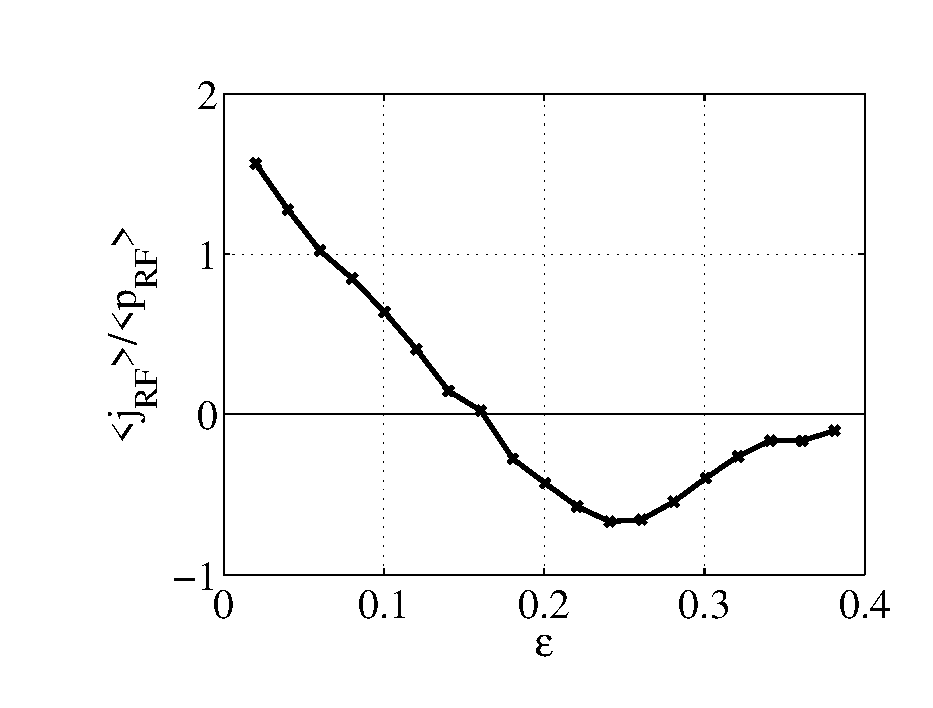
\includegraphics[width = 2in,height = 1in]{figures/test4_CST_ia_eta.eps}\\
(e)\hspace{1cm}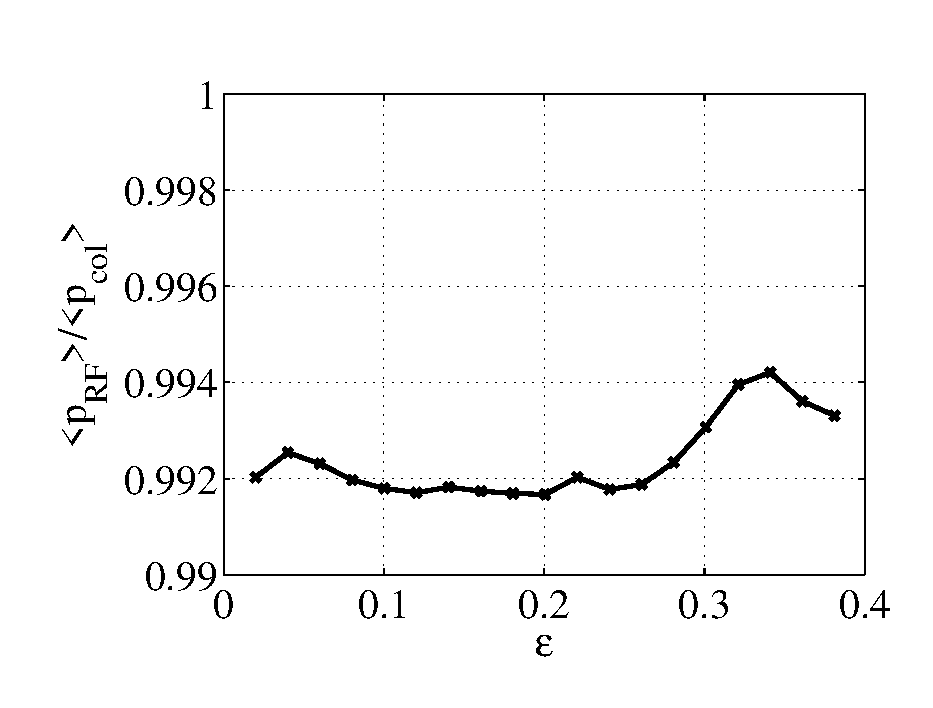
\includegraphics[width = 2in,height = 1in]{figures/test4_CST_ia_rf_col.eps}\\
\caption{ECCD in DIII-D ($D_{\text{EC}} = 0.15,\ N_{\parallel} =
0.3,\ Y = 0.98$). Output density (a), normalized current density
(b), normalized absorbed power density (c), normalized current
drive efficiency (d), ratio of power absorbed to power lost on
collisions (e), as a function of the inverse aspect ratio
$\epsilon = r/R_p$; temperatures, densities and $Z_{\text{eff}}$
are kept constant across the plasma.}
%\label{ebw_es}
\end{center}
\end{figure}

\begin{figure}[htb]
\begin{center}
(a)\hspace{1cm}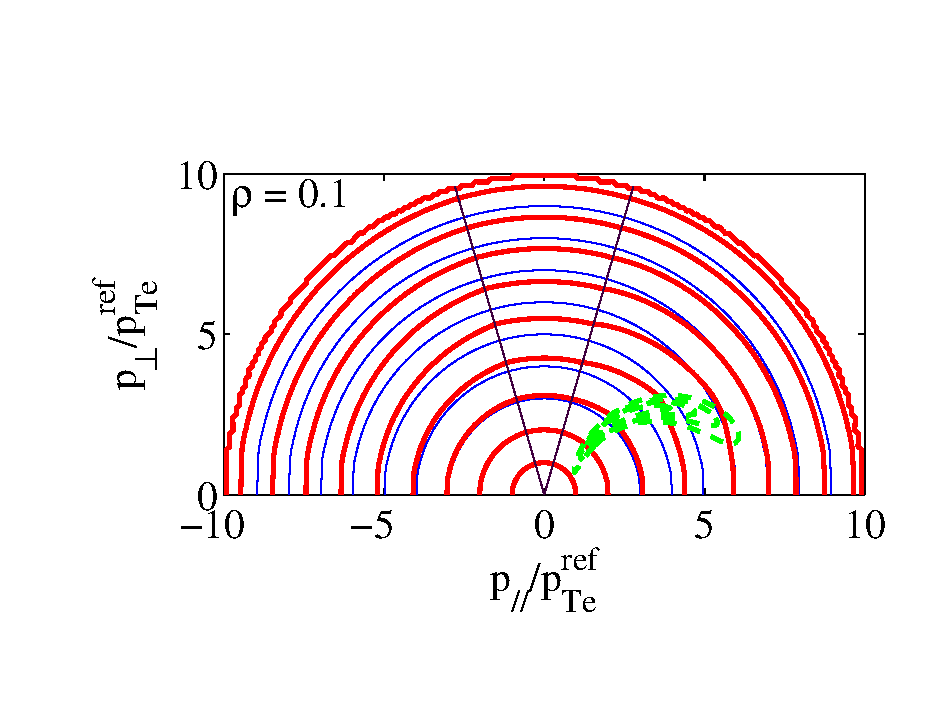
\includegraphics[width = 4in,height = 3in]{figures/D3D_test4_CST_f.eps}\\
(b)\hspace{1cm}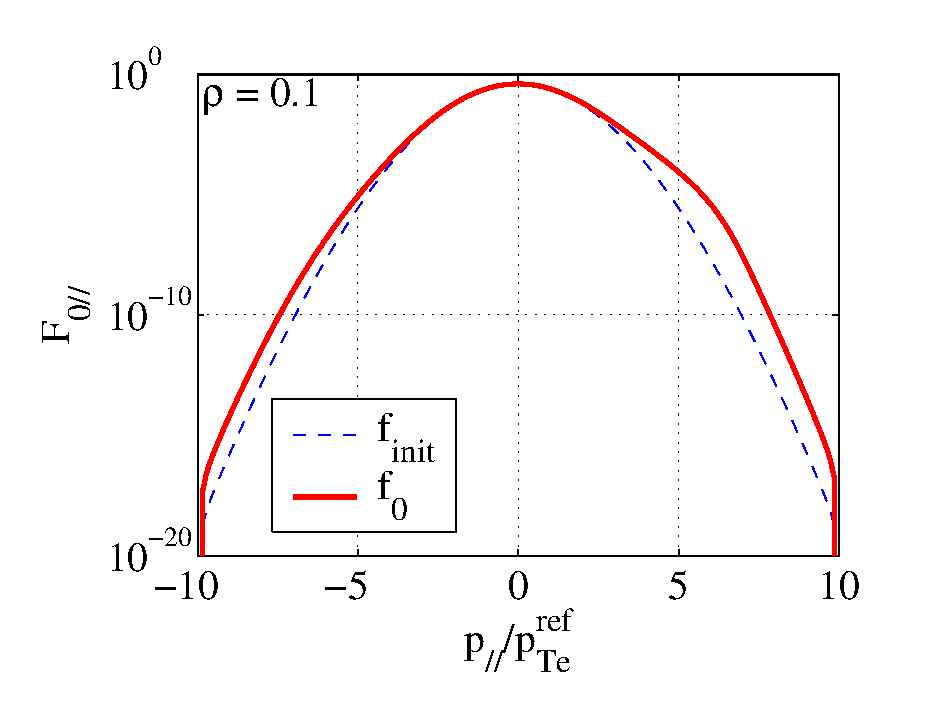
\includegraphics[width = 4in,height = 3in]{figures/D3D_test4_CST_fpar.eps}\\
(c)\hspace{1cm}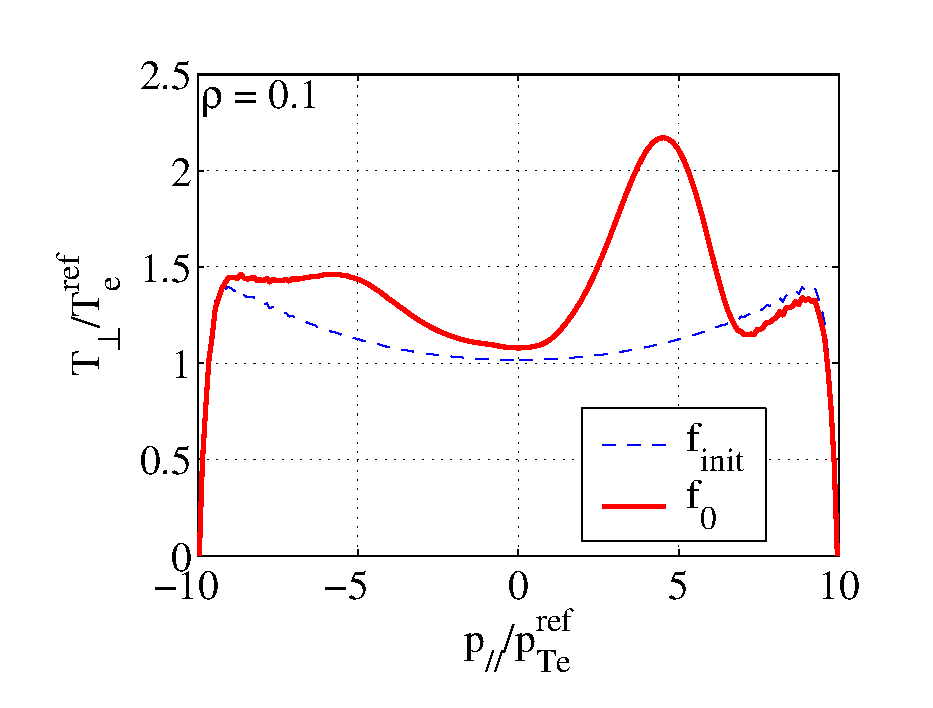
\includegraphics[width = 4in,height = 3in]{figures/D3D_test4_CST_tperp.eps}\\
\caption{ECCD in DIII-D ($\rho = 0.1,\ D_{\text{EC}} = 0.15,\
N_{\parallel} = 0.3,\ Y = 0.98$). 2D electron distribution
function (a), parallel distribution function (b) and perpendicular
temperature (c); blue thin lines represent $f_{\text{init}}$, red
thick lines represent $f_0$, and green dashed contours represent
$D_{\text{EC}}$.}
%\label{ebw_es}
\end{center}
\end{figure}

\begin{figure}[htb]
\begin{center}
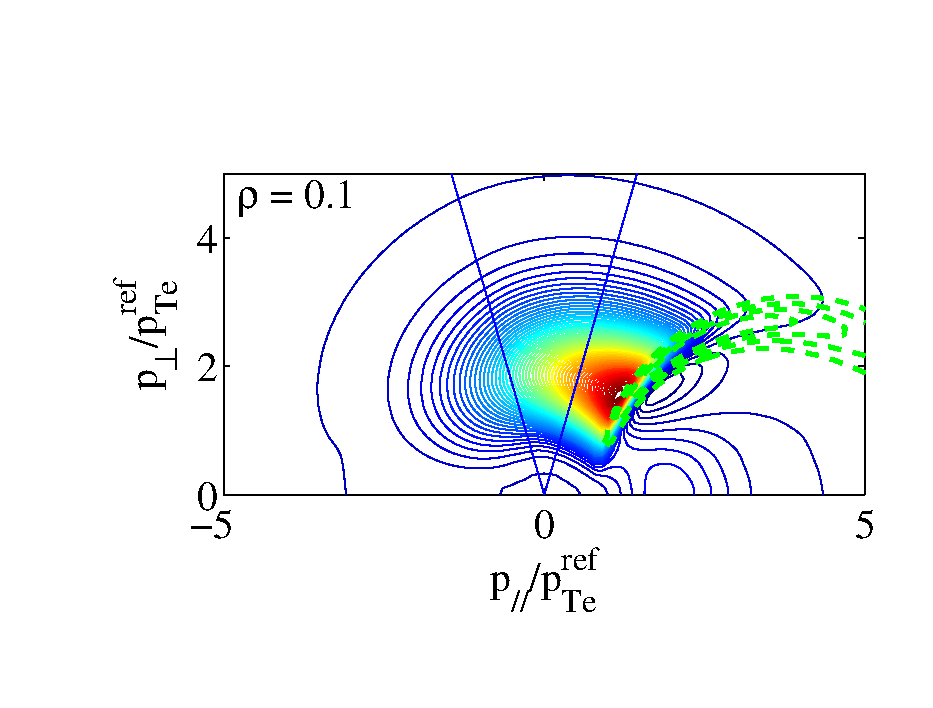
\includegraphics[width = 4in,height = 3in]{figures/D3D_test4_CST_A.eps}
\caption{ECCD in DIII-D ($\rho = 0.1,\ D_{\text{EC}} = 0.15,\
N_{\parallel} = 0.3,\ Y = 0.98$). Stream function for the momentum
space fluxes. Green dashed contours represent $D_{\text{EC}}$.}
%\label{ebw_es}
\end{center}
\end{figure}

\begin{figure}[htb]
\begin{center}
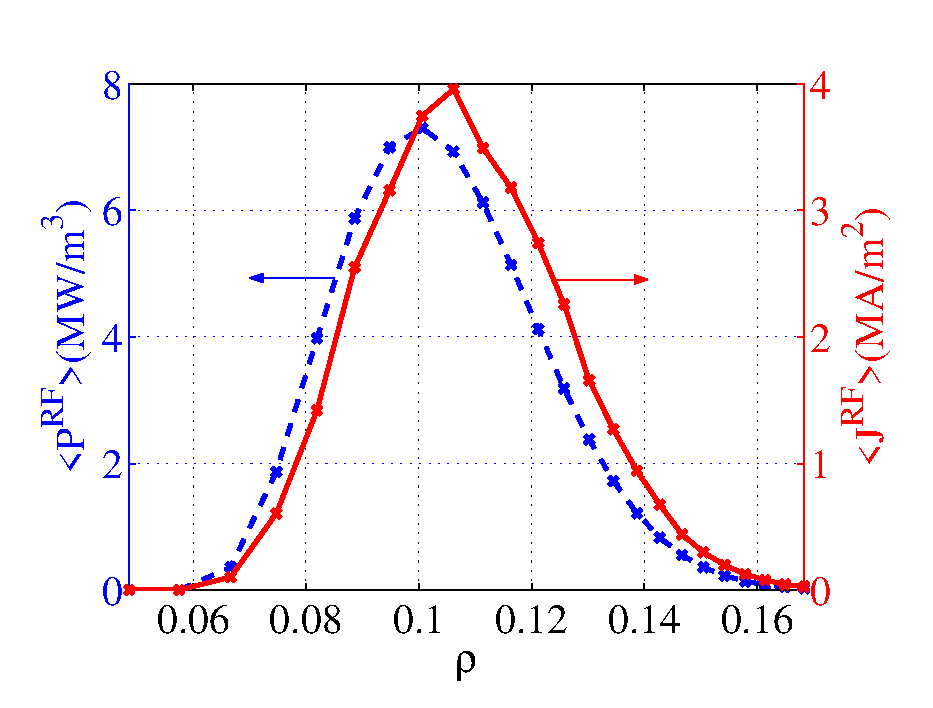
\includegraphics[width = 4in,height = 3in]{figures/JP_test4_030_110.eps}
\caption{ECCD in DIII-D ($\theta_b = 0,\ P_{\text{EC}} = 1 \text{
MW},\ N_{\parallel} = 0.3,\ f_{\text{EC}} = 110 \text{ MHz}$).
Current and power densities deposition profiles. 3D calculation
with $n_p = n_{\xi} = 100, n_{\psi} = 26$.}
%\label{ebw_es}
\end{center}
\end{figure}
